\subsection{Aproximación cuasiestática}
\subsubsection{Dipolo eléctrico (caso estático)}

En electrodinámica clásica, se entiende como \textit{límite cuasiestático} el considerar una partícula de tamaño mucho menor que la longitud de onda de la luz incidente \cite{Cuasiest}. En el caso de un elipsoide caracterizado por una función dieléctrica $\epsilon_p$, que se encuentra inmerso en un medio caracterizado por una función dieléctrica $\epsilon_m$ y cuyo semieje mayor es $a$, se puede definir el límite cuasiestático cuando el parámetro de tamaño $x=ka$ es mucho menor que la unidad \cite{Bohren}, donde $k=2\pi \sqrt{\epsilon_m}/\lambda$. Esta aproximación garantiza que toda la geometría del elipsoide esté sujeta a un campo eléctrico de la misma intensidad y dirección. \cite{Miguel}\\


En la aproximación cuasiestática, es posible analizar a la partícula mediante la aproximación dipolar. Para ello, es necesario estudiar un \textit{dipolo físico}, el cual puede considerarse como un \textit{dipolo eléctrico puntual} al aplicar un límite específico en su configuración. Un dipolo físico consiste en dos cargas puntuales $q$ y $-q$ separadas a una distancia $d$, con momento dipolar $\Vec{p}=p\hat{e}_z$ donde $p=qd$. Si las cargas se encuentran embebidas en un medio homogéneo e infinito con función dieléctrica $\epsilon_m$ y están localizadas a una distancia $r_{\pm}$ de $\Vec{r}$, donde $r_{+}$ corresponde a la distancia entre $q$ y $\Vec{r}$, y $r_{-}$ a la distancia entre $-q$ y $\Vec{r}$, el potencial  electrostático $\phi$ producido por el dipolo físico evaluado en $\Vec{r}$ está dado por \cite{Bohren,Griffiths}:
\begin{equation}
    \phi(\Vec{r})=\frac{q}{4\pi\epsilon_m}\left(\frac{1}{r_+}-\frac{1}{r_{-}}\right),    
\end{equation}
donde, al emplear la ley de cosenos con $\cos\theta=\Vec{r}\cdot\hat{e}_z/r$,
\begin{equation*}
	r_{\pm}=r^2+\left(\frac{d}{2}\right)^2\mp r\:d\cos\theta=r^2\left(1\mp\frac{d}{r}\cos\theta+\frac{d^2}{4r^2}\right).
\end{equation*}
Al evaluar el potencial en $r\gg d$, se desprecian los términos de segundo orden de $r/d$ y al realizar una expansión en serie de Taylor de un binomio, se obtiene:
\begin{equation}
    \frac{1}{r_+}-\frac{1}{r_{-}}\approx\frac{1}{r}\left(1+ \frac{\Vec{r}\cdot\hat{e}_z}{2r^2}d-1+ \frac{\Vec{r}\cdot\hat{e}_z}{2r^2}d\right)\approx\frac{1}{r}\left( \frac{\Vec{r}\cdot\hat{e}_z}{r^2}d\right)=\frac{\Vec{r}\cdot\hat{e}_z}{r^3}d.    
\end{equation}
Al considerar la aproximación dipolar, es decir, aproximar a $d$ igual a cero de tal forma que $qd$ permanezca constante \cite{Bohren}, se obtiene el potencial para un dipolo puntual:
\begin{equation}
\phi=\frac{p}{4\pi\epsilon_m}\left(\frac{\Vec{r}\cdot\hat{e}_z}{r^3}\right)=\frac{\Vec{p}\cdot\Vec{r}}{4\pi\epsilon_m r^3}=\frac{p\cos\theta}{4\pi\epsilon_m r^2}.
\label{pot_dipolo}
\end{equation}

\begin{figure}[h!]
	\centering
	\includegraphics[width=4.2cm]{../../Figuras/aproxdipolar}
	\caption{Esquema de un dipolo físico. Se muestran dos cargas puntuales $q$ y $-q$ separadas a una distancia $d$. La distancia entre $\Vec{r}$ y las cargas $q$ y $-q$ está dada por $r_+$ y $r_{-}$, respectivamente. }
	\label{dipolo_elec}
\end{figure}

\subsubsection{Dipolo eléctrico (caso dinámico)}
Los campos electromagnéticos presentan diferentes propiedades propiedades según la región en la que se encuentren. Al considerar las dimensiones de la fuente  del orden $d$ y la longitud de onda $\lambda=2\pi c/\omega$, entonces hay tres regiones de interés: la región cercana (estática) en donde $d\ll r\ll\lambda$, que se estudió en la sección anterior, la región intermedia en donde $d\ll r\sim \lambda$ y la región lejana (de radiación) donde $d\ll \lambda\ll r$.

El potencial de la sección anterior considera que las cargas se encuentran fijas en el espacio y están sometidas a un campo eléctrico homogéneo. Este potencial correspondería al de la partícula elipsoidal con una polarización $p$ a determinar en presencia de un campo eléctrico homogéneo alineado en la dirección $\hat{e}_z$. El siguiente escenario a considerar es de las cargas moviéndose en presencia de un campo eléctrico dinámico. Una forma de solucionar este problema es considerar que el movimiento de los campos, y por lo tanto de las cargas y corrientes, es armónico; lo cual es equivalente a realizar un análisis en componentes de Fourier de cualquier movimiento. De esta forma, no se pierde generalidad de considerar a los potenciales y campos de un sistema de cargas y corrientes localizadas en el espacio vacío, con una dependencia armónica variando en el tiempo y que oscilan a la frecuencia $\omega$ del campo electromagnético aplicado \cite{Jackson}
\begin{align}
    \rho(\Vec{r},t)&=\rho(\Vec{r})e^{-i\omega t},\nonumber\\
    \Vec{J}(\Vec{r},t)&=\Vec{J}(\Vec{r})e^{-i\omega t},
    \label{armonicf}
\end{align}
considerando que el significado físico lo posee la parte real. Por consiguiente, las Ecuaciones de Maxwell están dadas por
\begin{align}
	\nabla\cdot\Vec{E}&=\frac{\rho}{\epsilon_0},\\
	\nabla\cdot\Vec{H}&=0,\\
	\nabla\times\Vec{E}&=i\omega\mu_0\Vec{H},\\
	\nabla\times\Vec{H}&=\Vec{J}-i\omega\epsilon_0\Vec{E},
\end{align}
donde $\Vec{B}=\nabla\times\Vec{A}$, con $\Vec{A}$ el potencial vectorial y $ \Vec{H}=\Vec{B}/\mu_0$. Entonces,
\begin{equation}
	\Vec{H}=\frac{1}{\mu_0}\nabla\times\Vec{A}\hspace{0.5cm}\mbox{y}\hspace{0.5cm}    \Vec{E}=\frac{i}{\omega\epsilon}\nabla\times\Vec{H}.
\end{equation}

Si se consideran fuentes armónicas en el tiempo [Ec. (\ref{armonicf})], es posible determinar los campos electromagnéticos mediante el potencial vectorial como \cite{Jackson}:
\begin{align*}
  \Vec{A}(\Vec{r},t)=\frac{\mu_0}{4\pi}\int d^3r'\frac{\Vec{J}(\Vec{r'})e^{i\omega \frac{|\Vec{r}-\Vec{r'}|}{c}}}{|\Vec{r}-\Vec{r'}|}e^{-i\omega t},
\end{align*}
en donde se emplea la norma de Lorentz \cite{Griffiths} y la densidad de corriente se evalúa en el tiempo de retardo $t_r=t-|\Vec{r}-\Vec{r'}|/c$. Sea $k=\omega/c$ y omitiendo la dependencia temporal
\begin{equation}
    \Vec{A}(\Vec{r},t)=\frac{\mu_0}{4\pi}\int \Vec{J}(\Vec{r'})\frac{e^{ik|\Vec{r}-\Vec{r'}|}}{|\Vec{r}-\Vec{r'}|} d^3r'.
    \label{pot_vectorial}
\end{equation} 

Para la región de campo cercano donde $r\ll\lambda$ (o $kr\ll 1$) la exponencial del potencial vectorial [Ec.\ref{pot_vectorial}] se aproxima a la unidad y con ello encontramos la expresión conocida de este \cite{Jackson}
\begin{equation*}
	\Vec{A}(\Vec{r},t)=\frac{\mu_0}{4\pi}\int \frac{\Vec{J}(\Vec{r'})}{|\Vec{r}-\Vec{r'}|} d^3r'.
\end{equation*} 


En la región de campo lejano ($kr\gg 1$) dado que la exponencial oscila rápidamente, determina el comportamiento del potencial vectorial. En esta región es suficiente aproximar

\begin{equation}
	|\Vec{r}-\Vec{r'}|\simeq r-\hat{e}_r\cdot\Vec{r'},    
\end{equation}
con $\hat{e}_r$ un vector unitario en la dirección de $\Vec{r}$. \footnote{Usando la ley de cosenos y haciendo una expansión binomial $
	|\Vec{r}-\Vec{r'}|=\sqrt{r^2+(r')^2-2rr'\cos\theta}=r\sqrt{1+\left(r'/r\right)^2-2\left((r'/r)\cos\theta\right)}\simeq r\left\{1-(\hat{e}_r\cdot\Vec{r'}/r)+1/2\left(r'/r\right)^2\right\}\simeq r-\hat{e}_r\cdot\Vec{r'}.$}
	
\begin{figure}[h!]
	\includegraphics[width=6cm]{../../Figuras/aprox}
	\caption{Vectores de posición $\Vec{r},\Vec{r'}$ del elemento de volumen dV y del punto P, respectivamente. Se muestra la distancia $|\Vec{r}-\Vec{r'}|$ entre estos últimos. }
\end{figure}
 Más aún, considerando la región de campo lejano, si sólo se consideran los términos que decaen como $r^{-1}$, el inverso de la distancia en la Ec.(\ref{pot_vectorial}) puede ser reemplazada por $r$. Entonces, el potencial vectorial es
\begin{equation*}
    \lim_{kr\rightarrow\infty}\Vec{A}(\Vec{r})=\frac{\mu_0}{4\pi}\frac{e^{ikr}}{r}\int \Vec{J}(\Vec{r'})e^{-ik\hat{e}_r\cdot\Vec{r'}}d^3r',    
\end{equation*}
que se puede reescribir al realizar la expansión en serie de potencias de la exponencial dentro de la integral de volumen, dando como resultado
\begin{equation*}
    \lim_{kr\rightarrow\infty}\Vec{A}(\Vec{r})=\frac{\mu_0}{4\pi}\frac{e^{ikr}}{r}\sum_n\frac{(-ik)^n}{n!}\int \Vec{J}(\Vec{r'})(\hat{e}_r\cdot\Vec{r'})^n d^3r'.    
\end{equation*}
Al considerar únicamente el primer término de la expansión como una primera aproxmación, se concluye que 
\begin{equation}
    \Vec{A}(\Vec{r})\approx\frac{\mu_0}{4\pi}\frac{e^{ikr}}{r}\int \Vec{J}(\Vec{r'}) d^3r',    
    \label{aprox_pot_vec}
\end{equation}
integrando por partes, \footnote{acá hay que hacer lo de la notación de tensores}
\begin{equation}
	\int\Vec{J}d^3r'=-\int \Vec{r'}(\nabla'\cdot\Vec{J})d^3r'=-i\omega\int \Vec{r'}\rho(\Vec{r'})d^3r',
	\label{Jrho}
\end{equation}
de donde se usa la ecuación de continuidad 
\begin{equation*}
    \nabla\cdot\Vec{J}=-\frac{\partial\rho}{\partial t}=i\omega\rho(\Vec{r}). 
\end{equation*}
Al sustituir la Ec.(\ref{Jrho}) en la Ec.(\ref{aprox_pot_vec}) y usando la definición del momento dipolar
\begin{equation*}
	\Vec{p}=\int \Vec{r'}\rho(\Vec{r'})d^3r',
\end{equation*}
se tiene que 
\begin{equation}
    \Vec{A}(\Vec{r})=-\frac{i\omega\mu_0}{4\pi}\frac{e^{ikr}}{r}\int \Vec{r'}\rho(\Vec{r'})d^3r'=-\frac{i\omega\mu_0}{4\pi}\frac{e^{ikr}}{r}\Vec{p} , 
    \label{A_dip}  
\end{equation}
con $\Vec{p}$ el momento dipolar eléctrico. Al calcular el campo H como el rotacional de $A/\mu$, y emplando la ley de Faraday-Lenz para determinar el campo eléctrico, se concluye que \footnote{Ver Apéndice A para el desarrollo de estas expresiones}
\begin{align}
	\Vec{E}&=\frac{i}{\omega\epsilon}\nabla\times\Vec{H}=\frac{1}{4\pi\epsilon_0}\left\{k^2(\hat{e}_r\times\Vec{p})\times\hat{e}_r\frac{e^{ikr}}{r}+[3\hat{e}_r(\hat{e}_r\cdot\Vec{p})-\Vec{p}]\left(\frac{1}{r^3}-\frac{ik}{r^2}\right)e^{ikr}\right\},\\
    \Vec{H}&=\frac{1}{\mu_0}\nabla\times\Vec{A}=\frac{ck^2}{4\pi}(\hat{e}_r\times\Vec{p})\frac{e^{ikr}}{r}\left(1-\frac{1}{ikr}\right).    
\end{align}
Obsérvese que el campo $\Vec{H}$ es transversal al vector radial para cualquier distancia, mientras el campo eléctrico tiene componentes paralelas y perpendiculares a $\hat{e}_r$.\\

\noindent En la zona de radiación cuando $kr\gg 1$ se tiene que \begin{align}
    \Vec{E}&=\sqrt{\frac{\mu_0}{\epsilon_0}}\Vec{H}\times\hat{e}_r=\frac{ck^2}{4\pi}(\hat{e}_r\times\Vec{p})\times\Vec{e}_r\frac{e^{ikr}}{r}=\frac{e^{ikr}}{-ikr}\frac{ik^3}{4\pi\epsilon_m}\hat{e}_r\times(\hat{e}_r\times\Vec{p}),\label{campoE}\\
    \Vec{H}&=\frac{ck^2}{4\pi}(\hat{e}_r\times\Vec{p})\frac{e^{ikr}}{r}.\label{campoH}  
\end{align}
Con base en la Ec. (\ref{A_dip}) al iluminar el sistema con una onda plana monocromática de frecuencia angular $\omega$, el dipolo inducido $p$ [Ec. (16)] y por tanto los campos electromagnéticos $\Vec{E}$ y $\Vec{H}$ [Ecs. (\ref{campoE}) y (\ref{campoH})] oscilarán a esa misma frecuencia. Por lo tanto, los campos electromagnéticos esparcidos $\Vec{E}_{s}$ y $\Vec{H}_{s}$, generados por el dipolo inducido, son
\begin{align}
    \Vec{E}_{s}&=\frac{e^{ikr}}{-ikr}\frac{ik^3}{4\pi\epsilon_m}\hat{e}_r\times(\hat{e}_r\times p) e^{i\omega t},\\
    \Vec{H}_{s}&=\frac{ck^2}{4\pi}(\hat{e}_r\times\Vec{p})\frac{e^{ikr}}{r}e^{i\omega t}.
\end{align}
 Sustituyendo el momento dipolar de un dipolo puntual $\Vec{p}=\epsilon_m \alpha E_0 e^{-i\omega t}\hat{e}_x$, se pueden reescribir a los campos esparcidos como
 \begin{align}
 	\Vec{E}_{s}&=\frac{e^{ikr}}{-ikr}\frac{ik^3}{4\pi\epsilon_m}\left(\epsilon_m \alpha E_0 \right)\hat{e}_r\times(\hat{e}_r\times \hat{e}_x)=\frac{e^{ik(r-z)}}{-ikr}\frac{ik^3}{4\pi}\left( \alpha E_0 e^{ikz}\right)\hat{e}_r\times(\hat{e}_r\times \hat{e}_x)=\frac{e^{ik(r-z)}}{-ikr}\Vec{X}E,
 	\label{E_scat}\\
 	\Vec{H}_{s}&=\frac{k}{\omega\mu}\hat{e}_r\times\Vec{E}_{s}.
 	\label{H_scat}
 \end{align}
donde $E=E_0 e^{ikz}$ y $\Vec{X}=\frac{ik^3}{4\pi}\alpha \hat{e}_r\times(\hat{e}_r\times \hat{e}_x)$ es
el vector de amplitud de esparcimiento y su polarización en la base de vectores esféricos es $\Vec{p}=\epsilon_m \alpha E_0 e^{-i\omega t}(\sin\theta\cos\phi\: \hat{e}_r+\cos\theta\cos\phi\: \hat{e}_{\theta}-\sin\phi \:\hat{e}_{\phi})$ \footnote{Es decir, $\hat{e}_r\times(\hat{e}_r\times \hat{e}_x)=-\cos\theta\cos\phi \hat{e}_{\theta}+\sin\phi \hat{e}_{\phi}$. }. \\

